\section{Blockchain}
In diesem Kapitel wird auf die revolutionären Vorteile der Blockchain 
eingegangen, durch die diese Technologie Einzug in den Finanzsektor gewonnen 
hat. Dem werden im Nachgang die einhergehenden Nachteile und Risiken gegenübergestellt. 

\subsection{Aufbau und Funktionsweise einer Blockchain}
Um die Einsatzgebiete für eine Blockchain im Finanzsektor besser zu verstehen,
wird im Folgenden der Aufbau und die Komponenten grob dargestellt.
Ein elementarer Grundbaustein einer Blockchain ist die Bildung eines Hashes.
\glqq Eine Hash-Funktion bildet eine beliebig große Menge an Eingabedaten [...] auf eine Zahl von 
fixer Größe ab, den sogenannten Hashwert\grqq{} \cite[p.~6]{fill2020blockchain}.
Die Hash-Funktion soll darüber hinaus drei wichtige Eigenschaften besitzen.
Das Diffusionsprinzip beschreibt eine deutliche Änderung des Hashwertes bei einem leicht
abgeänderten Eingabewert. Dadurch können unterschiedliche Eingaben sofort erkannt werden.
Das Konfusionsprinzip beschreibt die Eigenschaft, dass vom Hashwert nicht auf den Eingabewert
geschlossen werden kann. Beim Vergleich zweier Hashwerte von Eingaben mit einer minimalen
Änderung kann nichtmal auf die Position der Abweichung geschlossen werden.
Zuletzt ist die Kollisionsresistenz insbesondere im Bereich der Kryptographie relevant.
Eine Kollision tritt dann auf, wenn zwei unterschiedliche Eingaben auf denselben Hash abgebildet
werden. // Die Hash-Funktion soll hierfür möglichst vermeiden zwei unterschiedliche Eingabewerte
auf denselben Hashwert abzubilden.
\cite[p.~6ff]{fill2020blockchain} 

Im Block 1 wird zuerst jeweils ein Hash H1 und H2 für die Datenpunkte Transaktion 1 
und Transaktion 2 gebildet. Aus diesen Hashes wird dann ein gemeinsamer Hash H12 gebildet, 
der den Block Header 1 darstellt.
Analog zum Block Header 1 wird Block Header 2 erstellt. Zusätzlich enthält dieser eine
Referenz auf den vorigen Block Header 1 und ist somit der Kopf der Kette. Der Block Header 2
kann weiterführend im Block Haeder 3 eines dritten Blocks referenziert werden. 
\ref{fig:BC_Aufbau}
Durch diese Datenstruktur kann ein involvierter Rechnerknoten die einzelnen Blöcke rekursiv
zurückverfolgen und Einblick in alle zuvor getätigten Transaktionen haben.
\cite[p.~17f]{fill2020blockchain}

\begin{figure}[h!]
    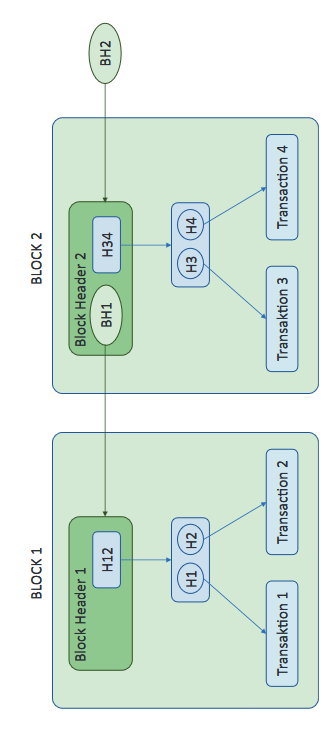
\includegraphics[width=\columnwidth]{BC_Aufbau.png}
    \quelle{\cite[p.~19]{fill2020blockchain}}
    \caption{Aufbau einer Blockchain \cite[p.~19]{fill2020blockchain}}
    \label{fig:BC_Aufbau}
\end{figure}

Damit ist die Blockchain ein verteiltes Register mit Integritätsgarantie. Die Integrität 
wird hierbei sichergestellt, indem eine Änderung an einem beliebigen Punkt in der
Blockchain eine Anpassung in allen Blöcken nach sich zieht, die eine direkte oder
indirekte Referenz auf diesen Block haben. Dank klarer und verschlüsselter Eigentumsansprüche
werden Änderungen nur dann vorgenommen, wenn sie berechtigt sind.
Als Schutzmechanismus werden Änderungen jedoch nur dann vorgenommen, wenn sie durch klare
und verschlüsselte Eigentumsansprüche berechtigt sind.
\cite[p.~22]{fill2020blockchain} 


\subsection{Einsatzgebiete im Finanzsektor}
Bereits ... hat die Blockchain ihren Einzug in den Finanzsektor gefeiert. Manche
Sektoren sind aufgrund der Blockchain neu entstanden, wie der Kryptomarkt. Andere Sektoren,
wie der Aktienmarkt wurden dadurch grundlegend/stark verändert. Wieder andere Bereiche, in denen die Blockchain
einen essentiellen Teil bildet, sind nicht sehr bekannt. Im Folgenden wird der Einfluss
der Blockchain auf zuvor vorhandene Finanzsektoren, sowie neu erschlossene Sektoren 
betrachtet.

\subsubsection{Transaktionen / Kryptowährungen}
Der Kryptomarkt ist der wohl bekannteste Bereich, in der die Blockchain ein 
grundlegender Bestandteil ist. 
Die stärksten Kryptowährungen sind Bitcoin und Ethereum. 
Die Blockchain gewährleistet die Sicherheit und Nachvollziehbarkeit von Transaktionen.
\cite[p.~168]{chowdhary2025smart}
Das wird dadurch erreicht, indem die Transaktionen fest in der Blockchain codiert sind.
 \cite[p.~11f]{pirafelnerblockchaintechnologie}
 Zusätzlich wird ein Konsensalgorithmus
 \cite[p.~32]{fill2020blockchain}

% Verweis auf vorher verifizierte Blöcke & vollst. Kopie auf jedem teilnehmenden Gerät.
Die Blockchain-Technologie ermöglicht einen Peer-to-Peer Austausch von digitalen
Währungseinheiten. Dadurch werden Zwischeninstanzen, wie Banken und andere Zahlungsdienstleister,
die die Vertrauenswürdigkeit der Transaktionsakteure beglaubigen sollen, nicht benötigt.
\cite[p.~32]{fill2020blockchain}



\subsubsection{Tokenization von Assets}

\subsubsection{Smart Contracts}
\cite[p.~14]{pirafelnerblockchaintechnologie}

\subsubsection{Smart Grid im Energiesektor}
% Besser im Kapitel Nachhaltigkeit!
\cite[p.~72]{fill2020blockchain}


\subsection{Risiken bei der Integration von Blockshains}
\cite[p.~17]{pirafelnerblockchaintechnologie}